\documentclass[border=10pt]{standalone}
\usepackage{tikz}
\usetikzlibrary{arrows.meta, positioning, calc}

\begin{document}
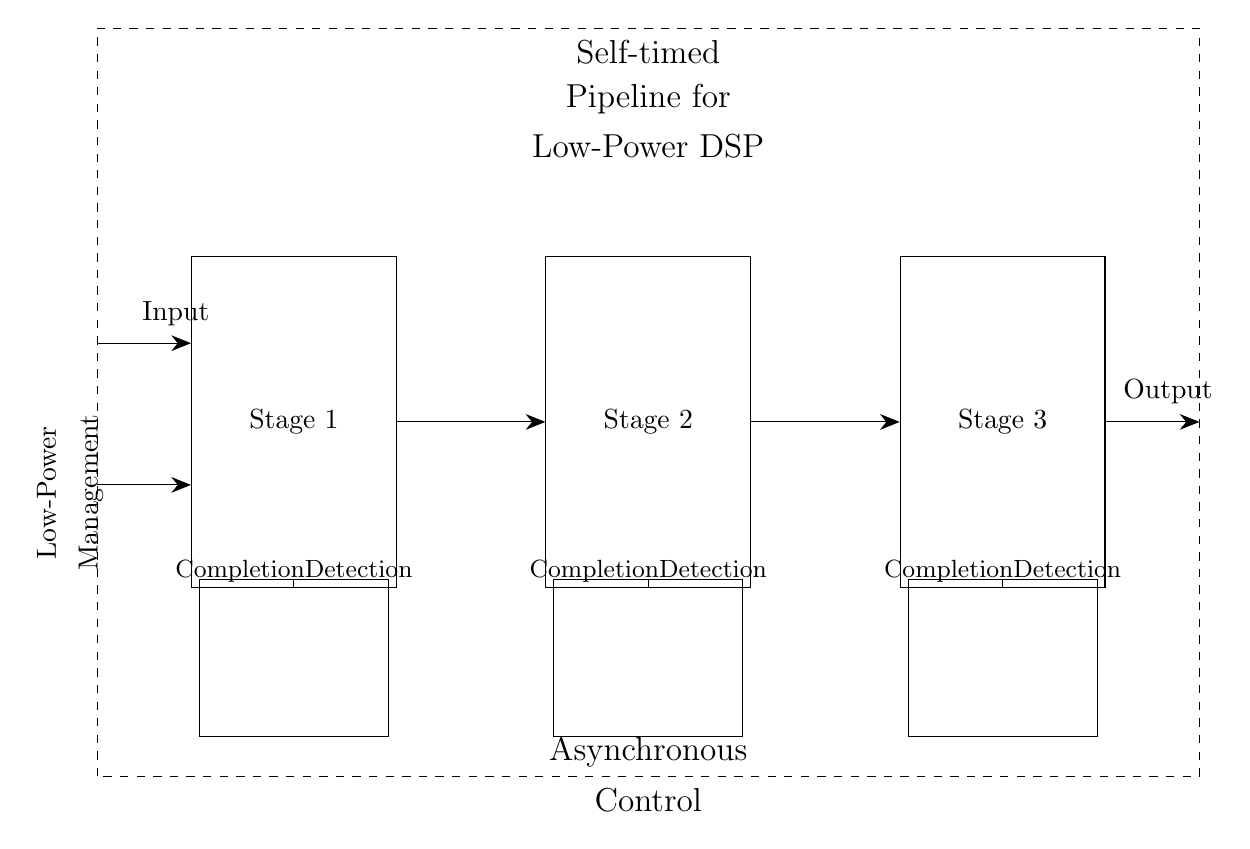
\begin{tikzpicture}[
  block/.style={draw, minimum width=2.6cm, minimum height=4.2cm},
  smallblock/.style={draw, minimum width=2.4cm, minimum height=2.0cm},
  >={Stealth[length=2.5mm,width=2mm]},
  font=\normalsize
]

% Outer dashed frame
\draw[dashed] (-1, -4.5) rectangle (13, 5);

% Title at top
\node[font=\large] at (6,4.7) {Self-timed};
\node[font=\large] at (6,4.1) {Pipeline for};
\node[font=\large] at (6,3.5) {Low-Power DSP};

% Bottom caption
\node[font=\large] at (6,-4.2) {Asynchronous};
\node[font=\large] at (6,-4.8) {Control};

% Main stage blocks
\node[block] (s1) at (1.5,0) {Stage 1};
\node[block] (s2) at (6,0) {Stage 2};
\node[block] (s3) at (10.5,0) {Stage 3};

% Horizontal connections between stages
\draw[->] (s1.east) -- (s2.west);
\draw[->] (s2.east) -- (s3.west);

% Input arrow on left to Stage 1
\draw[->] (-1,1) -- (s1.west|-0,1);
\node[anchor=south] at (0.0,1.1) {Input};

% Low-Power Management arrow (slightly lower)
\draw[->] (-1,-0.8) -- (s1.west|-0,-0.8);
\node[rotate=90, anchor=south] at (-1.4,-0.9) {Low-Power};
\node[rotate=90, anchor=south] at (-0.8,-0.9) {Management};

% Output arrow on right from Stage 3
\draw[->] (s3.east) -- (13,0);
\node[anchor=south] at (12.6,0.1) {Output};

% Completion detection small blocks under each stage
\node[smallblock] (c1) at (1.5,-3) {};
\node[smallblock] (c2) at (6,-3) {};
\node[smallblock] (c3) at (10.5,-3) {};

% Vertical connections from stage to completion detection
\draw (s1.south) -- (c1.north);
\draw (s2.south) -- (c2.north);
\draw (s3.south) -- (c3.north);

% Completion Detection label along bottom
\node[font=\small] at (1.5,-1.9) {CompletionDetection};
\node[font=\small] at (6,-1.9) {CompletionDetection};
\node[font=\small] at (10.5,-1.9) {CompletionDetection};

\end{tikzpicture}
\end{document}